\chapter{Experiments}

\section{Experimental Objective}

The main objective of the experiments conducted in this work is to analyse the impact of financial report sentiment on short-term stock price movements. More specifically, the experiments aim to determine whether incorporating sentiment-derived features from financial reports improves the predictive performance of machine learning models compared to models that rely solely on historical stock price indicators.

The prediction horizon considered in this work is the short term, ranging from one to seven trading days following the publication of a financial report. This interval was selected because financial disclosures are expected to influence market reactions shortly after becoming publicly available.

The experiments therefore compare two categories of models:

\begin{itemize}
\item models trained exclusively on stock market indicators derived from historical price and volume data (such as moving averages, momentum indicators and trading volume);
\item models trained on the same stock market indicators augmented with sentiment features extracted from financial reports.
\end{itemize}

The primary interest of this analysis is not to obtain the most accurate predictive model for stock price forecasting. Instead, the goal is to measure the relative performance improvement introduced by sentiment information. In other words, the experiments focus on observing the performance difference between models trained without sentiment features and models trained with sentiment features.

This comparison is performed across two prediction tasks, classification and regression, across multiple machine learning models and across prediction horizons ranging from one to seven days.

The resulting performance differences allow us to quantify whether textual sentiment extracted from financial reports provides additional predictive power beyond traditional market indicators.

\section{Evaluation Metrics}

In order to assess the predictive capabilities of the models, different evaluation metrics are used for the classification and regression tasks.

\subsection{Classification Metric}

For the classification task, the models predict one of three possible outcomes for the stock price movement:
\textit{UP}, \textit{STAY} or \textit{DOWN}.

Although accuracy is a commonly used metric for classification problems, it is not well suited for this task. The distribution of the three classes in the dataset is slightly imbalanced, meaning that some classes appear more frequently than others. In such situations, a model could achieve a deceptively high accuracy simply by favouring the majority class.

To address this issue, the experiments use the macro-averaged F1 score. The F1 score represents the harmonic mean between precision and recall, providing a balanced measure of a model's ability to correctly identify each class.

Precision and recall are defined as:

\begin{equation}
Precision = \frac{TP}{TP + FP}
\end{equation}

\begin{equation}
Recall = \frac{TP}{TP + FN}
\end{equation}

where $TP$ represents true positives, $FP$ false positives and $FN$ false negatives.

The F1 score is defined as:

\begin{equation}
F1 = 2 \cdot \frac{Precision \cdot Recall}{Precision + Recall}
\end{equation}

Since the problem involves three classes, the macro-average F1 score is used. This metric computes the F1 score independently for each class and then averages the results:

\begin{equation}
F1_{macro} = \frac{1}{K} \sum_{i=1}^{K} F1_i
\end{equation}

where $K$ represents the number of classes.

The macro-average ensures that each class contributes equally to the final score, preventing the majority class from dominating the evaluation metric.

\subsection{Regression Metric}

For the regression task, the goal is to predict the numerical return of the stock price after a given time horizon.

To evaluate regression performance, the Root Mean Squared Error (RMSE) is used. RMSE measures the square root of the average squared difference between predicted values and actual values.

Formally, RMSE is defined as:

\begin{equation}
RMSE = \sqrt{\frac{1}{N} \sum_{i=1}^{N} (y_i - \hat{y}_i)^2}
\end{equation}

where:
\begin{itemize}
\item $y_i$ represents the true value,
\item $\hat{y}_i$ represents the predicted value,
\item $N$ is the total number of observations.
\end{itemize}

RMSE is particularly suitable for financial prediction tasks because it penalizes large prediction errors more heavily than small ones. This property is desirable when predicting stock returns, as large errors may correspond to significant misestimations of market movement.

\section{Models}

The experiments employ three widely used machine learning models that represent different modelling paradigms: linear models, ensemble bagging methods, and gradient boosting methods.

\subsection{Logistic and Ridge Regression}

Logistic regression is used for the classification task, while ridge regression is used for the regression task. Both models belong to the family of linear models.

Linear models assume that the prediction can be expressed as a linear combination of the input features:

\begin{equation}
y = w_0 + \sum_{i=1}^{n} w_i x_i
\end{equation}

where $x_i$ are the input features and $w_i$ are the learned coefficients.

Logistic regression models the probability of each class using the logistic function and predicts the class with the highest probability. Ridge regression, on the other hand, extends linear regression by introducing an $L_2$ regularization term that penalizes large coefficients:

\begin{equation}
L = \sum_{i=1}^{N} (y_i - \hat{y}_i)^2 + \lambda \sum_{j=1}^{n} w_j^2
\end{equation}

This regularization helps reduce overfitting, especially when dealing with correlated features.

These models serve as simple and interpretable baselines that allow us to assess whether sentiment features provide additional predictive value even in relatively simple modelling frameworks.

\subsection{Random Forests}

Random Forest is an ensemble learning method based on decision trees. The model constructs a large number of decision trees during training and combines their predictions to produce the final output.

Each tree is trained on a random subset of the training data using a technique known as bootstrap sampling. Additionally, at each split in the tree, a random subset of features is considered. This randomness helps reduce correlation between individual trees and improves the generalization capability of the ensemble.

For classification tasks, the final prediction is obtained through majority voting among the trees. For regression tasks, the predictions of the trees are averaged.

Random forests are well suited for this problem because they can model nonlinear relationships between features and outcomes, while also being relatively robust to noise and feature interactions.

\subsection{XGBoost}

XGBoost (Extreme Gradient Boosting) is a gradient boosting framework that builds an ensemble of decision trees sequentially. Unlike random forests, which build trees independently, gradient boosting constructs each new tree in order to correct the errors made by the previous trees.

At each iteration, the algorithm fits a new tree to the residual errors of the current model. The final prediction is obtained by summing the contributions of all trees in the ensemble.

XGBoost includes several improvements over traditional gradient boosting algorithms, such as regularization, efficient handling of sparse data and optimized parallel computation. These properties make it one of the most widely used algorithms for structured tabular datasets.

Due to its ability to capture complex nonlinear relationships, XGBoost provides a strong benchmark for evaluating the usefulness of sentiment features in the prediction task.

\section{Hyperparameter Search}

Since the main objective of the experiments is not to obtain the best possible predictive model but rather to measure the impact of sentiment features, extensive hyperparameter tuning is not required.

Furthermore, computational resources available for this project are limited. For these reasons, only a modest grid search over a small set of hyperparameters is performed for each model.

This approach allows the models to reach a reasonable level of performance while keeping the computational cost manageable.

\section{Baseline Models}

In order to ensure that the evaluated models provide meaningful predictive power, their performance is compared against simple baseline predictors.

For the classification task, the baseline model always predicts the majority class observed in the training dataset. This baseline represents the simplest possible classifier and provides a lower bound for model performance.

For the regression task, the baseline model predicts the mean return observed in the training dataset for all observations. This corresponds to a constant predictor that ignores all input features.

Comparing machine learning models against these baselines ensures that the learned models capture patterns that go beyond trivial statistical properties of the dataset.

\section{Data Splitting Strategy}

In order to avoid information leakage and ensure that the experimental setup reflects a realistic forecasting scenario, the dataset is split according to time-series constraints. All observations are first sorted chronologically based on the filing date of the corresponding SEC report. The dataset is then divided into training, validation, and test sets such that observations in the training set occur strictly before those in the validation set, and validation observations occur before those in the test set.

This chronological ordering ensures that models are always trained using information available in the past and evaluated on future data, which is consistent with real-world financial prediction settings.

During model training, cross-validation is performed using an expanding window strategy. In this approach, the training window progressively increases as time advances, while the validation window moves forward accordingly. More formally, at each cross-validation step, the model is trained on all observations available up to a given time point and validated on the immediately following period.

This technique is particularly appropriate for financial time series because it preserves the temporal ordering of observations and allows the model to learn from progressively larger historical datasets while always being evaluated on unseen future data.

\section{Statistical Significance Testing}

To assess whether the inclusion of sentiment features leads to systematic improvements in predictive performance, statistical significance tests are conducted throughout the experimental evaluation. Because the experiments involve comparing two model configurations (with and without sentiment features) across multiple horizons or groups, paired statistical tests are employed. These tests evaluate whether the observed differences in performance are likely to arise from random variation or reflect a consistent improvement.

Let $\Delta_i$ denote the difference in performance between the model trained with sentiment features and the corresponding model trained without sentiment features for observation $i$. 
Depending on the experiment, each observation corresponds either to a prediction horizon or to a specific group (e.g., sector or industry). 
Positive values of $\Delta_i$ indicate that sentiment features improve predictive performance, whereas negative values indicate a degradation, for F1 score in classification, while for RMSE in regression, the opposite is true.

Three complementary statistical measures are reported:

\begin{itemize}
    \item \textbf{Mean improvement} $\bar{\Delta}$, which summarizes the average gain in performance attributable to sentiment features.
    
    \item \textbf{Confidence intervals}. A $95\%$ confidence interval for $\bar{\Delta}$ is computed in order to quantify the uncertainty associated with the estimated mean improvement. If the confidence interval does not include zero, this suggests that the effect is unlikely to be due to random fluctuations.
    
    \item \textbf{Hypothesis tests}. Two paired statistical tests are applied to evaluate whether the mean difference is significantly different from zero: the paired Student's $t$-test and the Wilcoxon signed-rank test.
\end{itemize}

\subsection{Paired Student's t-test}

The paired Student's $t$-test evaluates whether the mean of the paired differences $\Delta_i$ is statistically different from zero. Formally, the null hypothesis is defined as

\[
H_0 : \mathbb{E}[\Delta] = 0
\]

which states that the inclusion of sentiment features has no effect on predictive performance. The alternative hypothesis is

\[
H_1 : \mathbb{E}[\Delta] \neq 0 .
\]

The test statistic is computed as

\[
t = \frac{\bar{\Delta}}{s_\Delta / \sqrt{n}},
\]

where $\bar{\Delta}$ is the sample mean of the differences, $s_\Delta$ is the sample standard deviation of the differences, and $n$ is the number of paired observations. The resulting statistic is compared to a $t$-distribution with $n-1$ degrees of freedom to obtain a $p$-value.

The paired formulation is appropriate in this context because both model variants are evaluated on the same prediction tasks, ensuring that each pair of measurements is directly comparable.

\subsection{Wilcoxon Signed-Rank Test}

While the $t$-test assumes that the differences $\Delta_i$ are approximately normally distributed, this assumption may not always hold in practice, particularly when the number of observations is small. For this reason, the Wilcoxon signed-rank test is also applied as a non-parametric alternative.

The Wilcoxon test evaluates whether the median of the paired differences is significantly different from zero. Instead of relying on the raw values of $\Delta_i$, the test ranks the absolute values of the differences and analyzes the sum of the ranks associated with positive and negative signs. This procedure makes the test robust to deviations from normality and to the presence of outliers.

Using both the paired $t$-test and the Wilcoxon test provides a more reliable assessment of statistical significance, since the two tests rely on different assumptions about the underlying distribution of the performance differences.

\section{Normal and Adjusted Label Comparison}

The first suite of experiments evaluates the predictive performance of models across multiple forecasting horizons and different label formulations.
To investigate whether market-wide or industry-specific trends influence the predictive signal contained in financial reports, three different label definitions are considered:

\begin{itemize}
\item \textbf{Raw labels}: the original price movement labels based solely on the individual stock returns.
\item \textbf{Sector-adjusted labels}: returns adjusted relative to the average performance of the sector to which the company belongs.
\item \textbf{Industry-adjusted labels}: returns adjusted relative to the average performance of the more granular industry classification.
\end{itemize}

Comparing these three label formulations allows us to evaluate whether sentiment signals capture company-specific information or broader sector-level dynamics.

\subsection{Evolution of Sentiment Impact Across Prediction Horizons}

Figures \ref{fig:cls_logistic_delta}--\ref{fig:reg_xgb_delta} illustrate the evolution of the performance difference $\Delta$ between models trained with and without sentiment features across prediction horizons from one to seven days.
It can be seen that for the classification task, Logistic regression displays improved performance with sentiment features 
across all horizons for the raw labels, with the most pronounced improvement observed for the industry-adjusted labels. 
The improvement is generally more significant for longer horizons, particularly for 4-7 days.
While Random Forest and XGBoost lag behind, they still show the most improvement for the industry-adjusted labels.
For the regression task, Ridge regression exhibits the most consistent improvement across horizons for the industry-adjusted 
labels, while Random Forest and XGBoost show more mixed results with some horizons showing improvement and others showing deterioration when sentiment features are included.

\begin{figure}
\centering

% -------------------- Classification Row --------------------
\begin{subfigure}{0.32\textwidth}
\centering
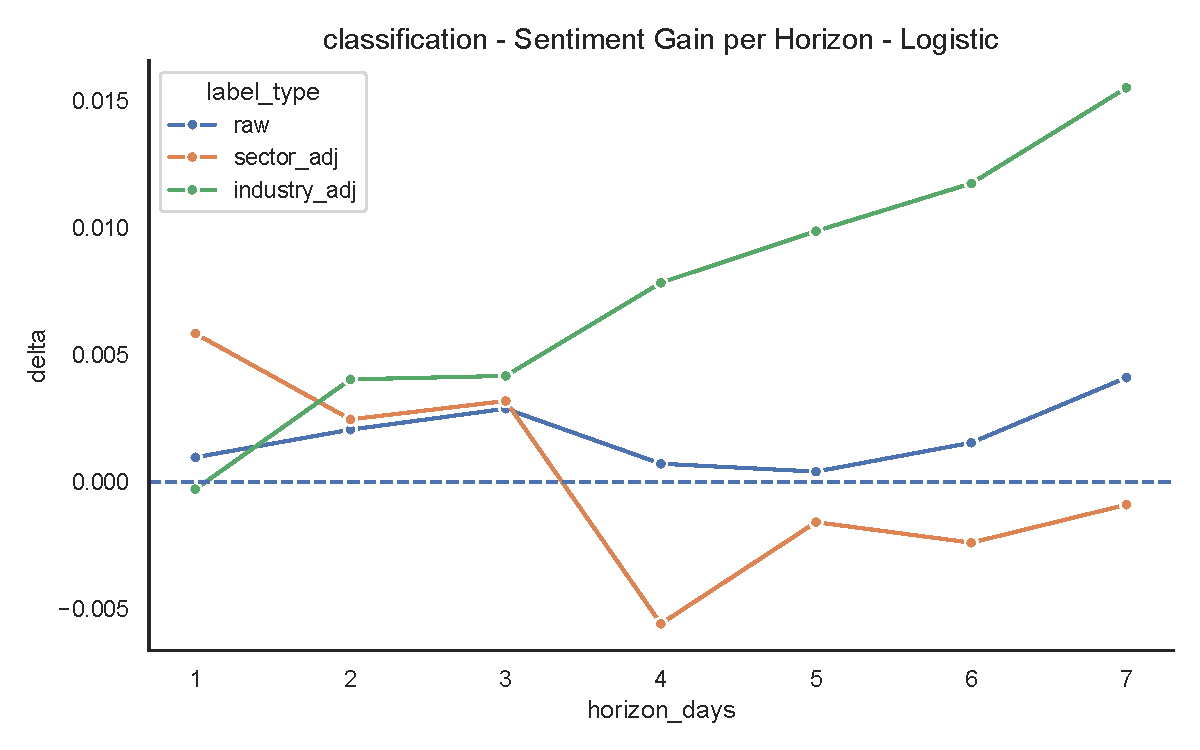
\includegraphics[width=\linewidth]{adjusted_comparison_images/comparison_classification_Logistic.pdf}
\caption{Logistic Regression}
\end{subfigure}
\hfill
\begin{subfigure}{0.32\textwidth}
\centering
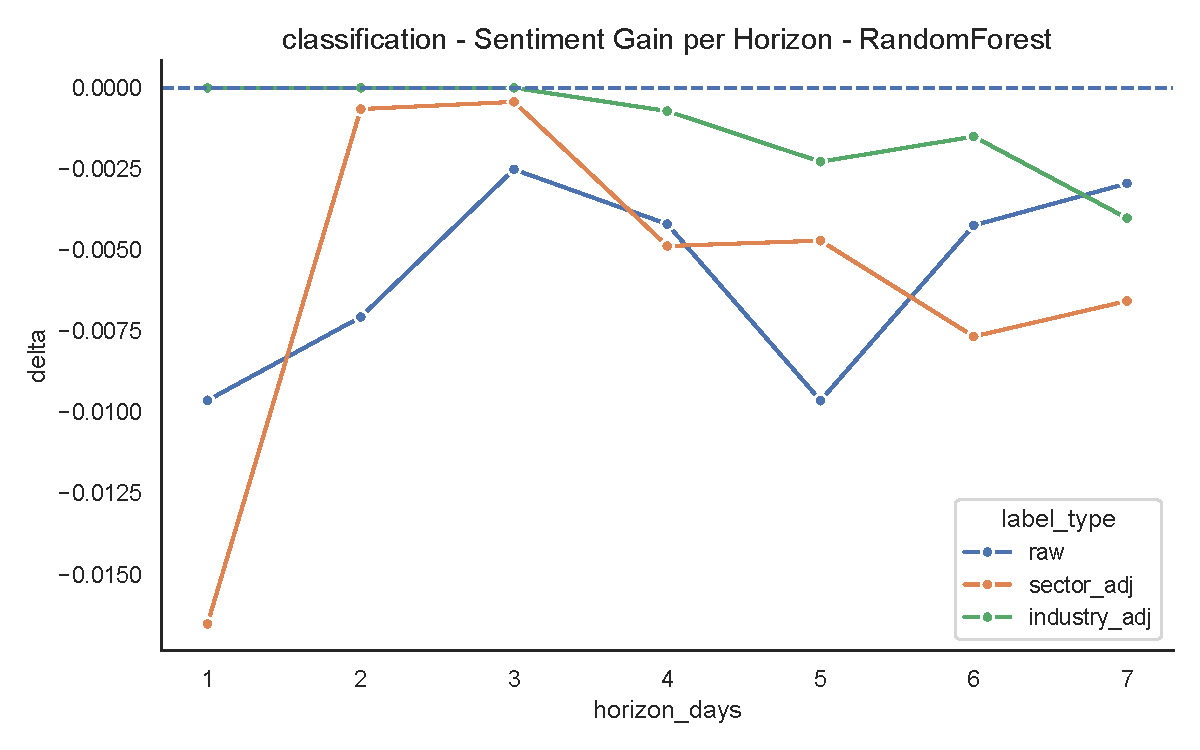
\includegraphics[width=\linewidth]{adjusted_comparison_images/comparison_classification_RandomForest.pdf}
\caption{Random Forest}
\end{subfigure}
\hfill
\begin{subfigure}{0.32\textwidth}
\centering
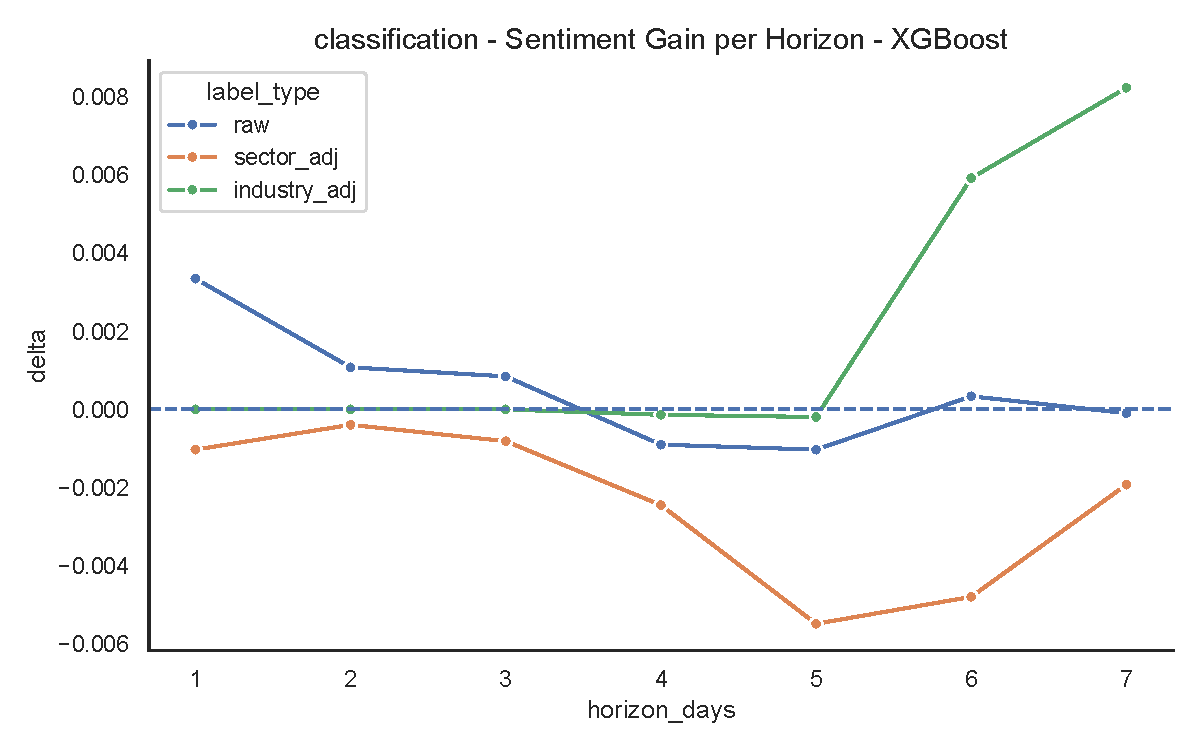
\includegraphics[width=\linewidth]{adjusted_comparison_images/comparison_classification_XGBoost.pdf}
\caption{XGBoost}
\end{subfigure}

\vspace{0.6cm}

% -------------------- Regression Row --------------------
\begin{subfigure}{0.32\textwidth}
\centering
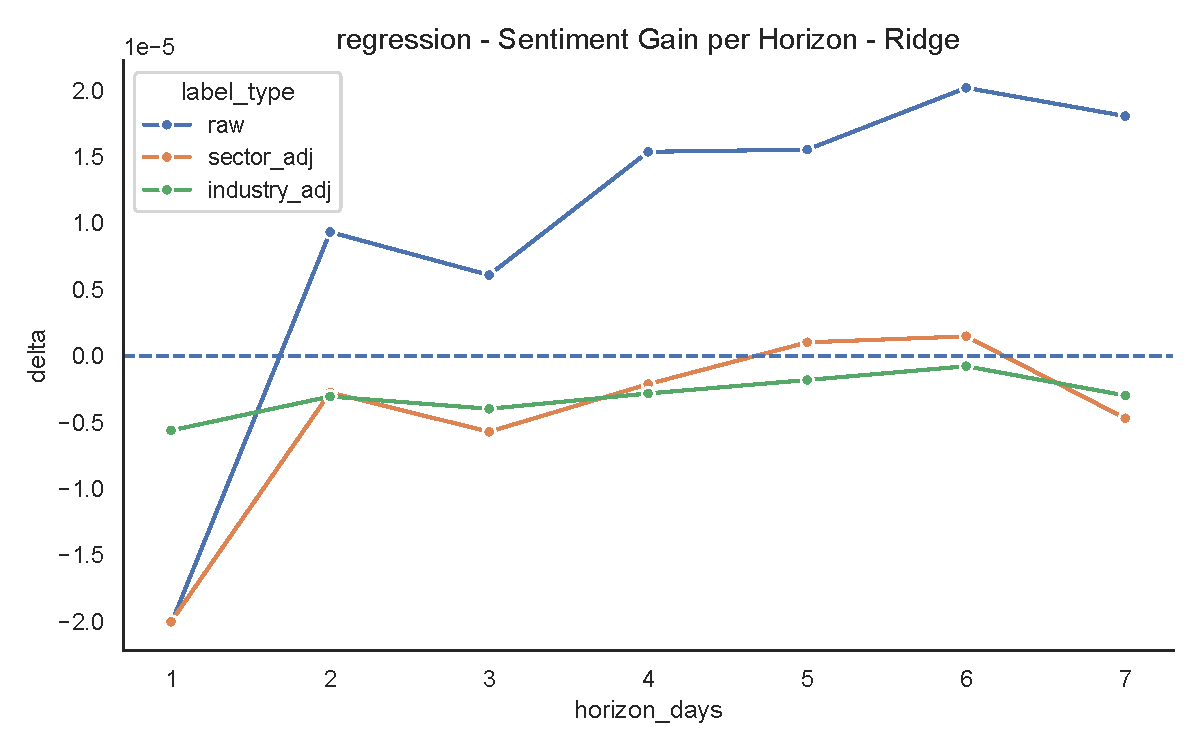
\includegraphics[width=\linewidth]{adjusted_comparison_images/comparison_regression_Ridge.pdf}
\caption{Ridge Regression}
\end{subfigure}
\hfill
\begin{subfigure}{0.32\textwidth}
\centering
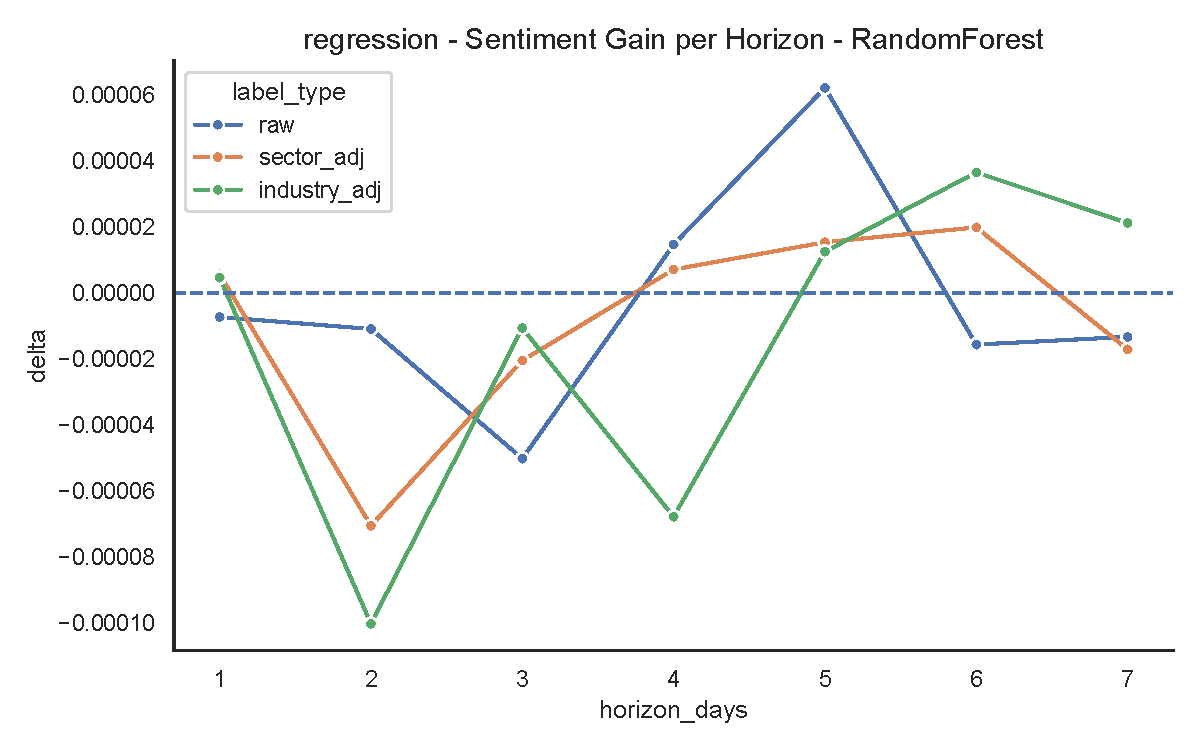
\includegraphics[width=\linewidth]{adjusted_comparison_images/comparison_regression_RandomForest.pdf}
\caption{Random Forest}
\end{subfigure}
\hfill
\begin{subfigure}{0.32\textwidth}
\centering
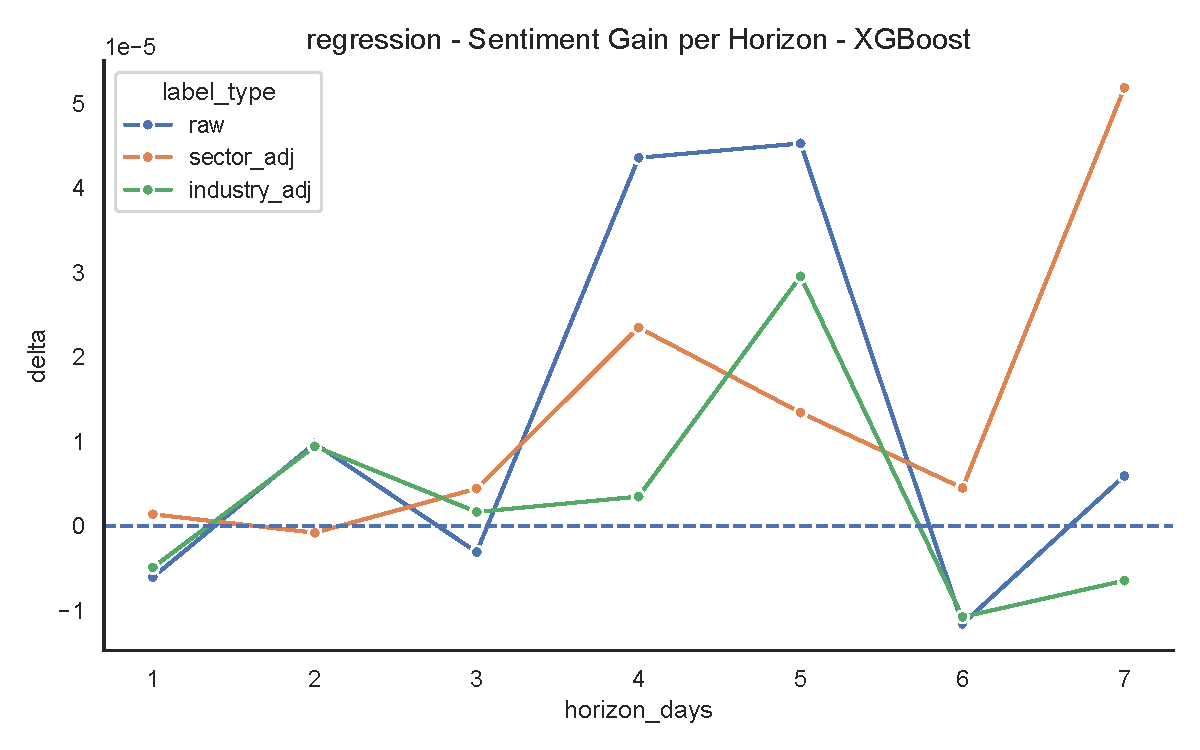
\includegraphics[width=\linewidth]{adjusted_comparison_images/comparison_regression_XGBoost.pdf}
\caption{XGBoost}
\end{subfigure}

\caption{Evolution of the sentiment contribution across prediction horizons for classification models (top row) and regression models (bottom row). Each subplot shows the mean performance delta when sentiment features are included compared to models trained without sentiment information. The blue line corresponds to raw labels, the orange line to sector-adjusted labels and the green line to industry-adjusted labels.}
\label{fig:sentiment_model_comparison}
\end{figure}

\subsection{Statistical Significance of Sentiment Contribution}

In this setting, the paired differences $\Delta_i$ correspond to the performance improvement obtained by adding sentiment features for each prediction horizon. Consequently, the number of paired observations used in the statistical tests is $n = 7$. The tests therefore assess whether sentiment features provide a consistent improvement across different forecasting horizons.
Confidence intervals and hypothesis tests are computed separately for each model and label type. This allows the analysis to determine not only whether sentiment features are useful overall, but also whether their effectiveness depends on how the target variable is defined.

\subsection{Classification Results}

For logistic regression, sentiment features lead to a small but statistically significant improvement when raw labels are used. The average improvement across the seven horizons is $\Delta = 0.0018$, with a $95\%$ confidence interval of $(0.0008, 0.0028)$. Both the paired $t$-test ($p = 0.011$) and the Wilcoxon signed-rank test ($p = 0.016$) indicate that the improvement is unlikely to be due to random variation. When sector-adjusted labels are used, the estimated effect becomes negligible ($\Delta = 0.0001$) and statistically insignificant, with the confidence interval spanning zero. In contrast, the improvement becomes more pronounced when industry-adjusted labels are employed. In this case the mean increase reaches $\Delta = 0.0076$, with a $95\%$ confidence interval of $(0.0036, 0.0115)$ and statistically significant $p$-values for both tests. This result suggests that sentiment features may capture company-specific signals that become more visible once broader industry movements are removed from the labels.

Random Forest models display a different behaviour. For raw labels, the inclusion of sentiment features leads to an average decrease in macro F1 score of $\Delta = -0.0058$, with a $95\%$ confidence interval of $(-0.0080, -0.0035)$ and statistically significant $p$-values ($p = 0.002$ for the $t$-test). A similar negative effect is observed when sector-adjusted labels are used, where the mean change is $\Delta = -0.0059$ and the confidence interval again excludes zero. For industry-adjusted labels the effect is smaller ($\Delta = -0.0012$) and no longer statistically significant. These results suggest that the tree-based ensemble may already capture complex nonlinear interactions in the market-based features, and the addition of sentiment signals may introduce noise rather than additional predictive information.

The results for XGBoost are more neutral. When raw labels are used, the average change in performance is very small ($\Delta = 0.0005$), and the corresponding confidence interval includes zero, indicating no statistically significant effect. When sector-adjusted labels are used, however, a small but statistically significant decrease in performance is observed ($\Delta = -0.0024$, $95\%$ CI $(-0.0039, -0.0009)$). For industry-adjusted labels, the estimated effect is again small and statistically insignificant. Overall, the results indicate that the interaction between gradient boosting models and sentiment-derived features may depend strongly on the specific label definition.

Despite these heterogeneous effects, all classification models outperform the trivial majority-class baseline by a substantial margin. Depending on the model and label type, the improvement over the baseline ranges from approximately $0.03$ to $0.18$ in macro F1 score. The associated statistical tests yield very small $p$-values in most cases, confirming that the models capture meaningful predictive patterns from the available feature set.

\subsection{Regression Results}

Across all regression models, the magnitude of the observed changes in RMSE is extremely small, typically on the order of $10^{-5}$. For Ridge regression with raw labels, the mean difference is $\Delta = 9 \times 10^{-6}$, and the corresponding confidence interval includes zero, indicating no statistically significant effect. When sector-adjusted labels are used, the average difference becomes slightly negative ($\Delta = -5 \times 10^{-6}$), but the statistical tests again fail to reject the null hypothesis.

A statistically significant change is observed only when Ridge regression is applied to industry-adjusted labels. In this case, the mean difference is $\Delta = -3 \times 10^{-6}$, with a $95\%$ confidence interval that excludes zero and statistically significant $p$-values for both the $t$-test and the Wilcoxon test. Although the effect is statistically detectable, its magnitude remains extremely small and therefore unlikely to be practically meaningful.

For the Random Forest regression model, the differences between models with and without sentiment features are consistently small and statistically insignificant across all label types. A similar pattern emerges for XGBoost regression. Although small variations in RMSE are observed across horizons, the corresponding confidence intervals always include zero and the hypothesis tests fail to detect statistically significant differences.

Nevertheless, all regression models perform at least comparably to the baseline mean predictor, and in some cases provide modest improvements in RMSE. However, the inclusion of sentiment features does not appear to materially influence predictive performance in this setting.

\subsection{Discussion}

Taken together, the results highlight several important patterns regarding the predictive value of sentiment features derived from financial reports.

First, the effect of sentiment features depends strongly on the model class. Linear models such as logistic regression appear to benefit the most from the additional textual information, particularly when industry-adjusted labels are used. In contrast, tree-based ensemble models often experience small decreases in classification performance when sentiment features are added. One possible explanation is that these models already capture complex nonlinear interactions within the structured market features, leaving limited room for additional improvement from textual signals.

Second, the choice of label definition plays a meaningful role in determining whether sentiment information is useful. The strongest improvements for logistic regression occur when industry-adjusted labels are used, suggesting that sentiment extracted from financial reports may capture company-level information that becomes more informative once broader industry movements are removed.

Finally, the results indicate a clear difference between classification and regression tasks. While sentiment features occasionally provide measurable improvements in classification performance, their impact on regression models predicting numerical returns is negligible. This finding is consistent with the intuition that textual sentiment may be more informative about the \emph{direction} of future price movements rather than the precise magnitude of those movements.

\section{Group-Specific Modeling: Company, Sector, and Industry Experiments}

In the previous experiments, models were trained on the full dataset containing filings from all companies. While this approach maximizes the number of available training samples, it implicitly assumes that the relationship between financial report sentiment and short-term stock price movements is homogeneous across companies and industries. In practice, however, market reactions to financial disclosures may differ substantially depending on firm-specific characteristics, sector dynamics, or industry structure.

To further investigate these effects, we conduct an additional experiment where models are trained and evaluated within different levels of grouping granularity. Specifically, three training scenarios are considered:

\begin{enumerate}
    \item \textbf{Company-level models.}  
    In this setting, a separate model is trained for each individual company (ticker). The training data consists exclusively of filings associated with that company, and performance is evaluated on the corresponding company-specific test set. This setup allows the model to capture firm-specific patterns in the relationship between textual sentiment and subsequent price movements. However, since the number of filings per company is relatively limited, the resulting models are expected to exhibit high variance and potentially unstable estimates.

    \item \textbf{Sector-level models.}  
    In the second configuration, one model is trained per economic sector. The training set aggregates filings from all companies belonging to that sector, and evaluation is performed on sector-specific test samples. Compared to the company-level setup, this configuration benefits from a substantially larger number of training examples while still preserving some degree of economic homogeneity. Sector-level modeling therefore represents a compromise between specialization and sample size.

    \item \textbf{Industry-level models.}  
    The third scenario lies between the previous two in terms of granularity. Here, models are trained separately for each industry classification. Industries are more specific than sectors but still contain multiple companies, leading to a moderate number of samples per group. This setup enables the analysis of whether sentiment extracted from financial reports carries predictive information within narrower business domains.
\end{enumerate}

Across all three settings, the same modeling framework described previously is applied. For each group (company, sector, or industry), models are trained both with and without sentiment features. 
The difference in predictive performance between these two configurations is denoted by $\Delta$, representing the performance gain attributable to the inclusion of textual sentiment features.

\subsection{Statistical Significance of Sentiment Contribution}

In this case, the paired differences $\Delta_i$ correspond to the performance improvement obtained by adding sentiment features within each group across the horizons.
For example, in the sector-level experiments each $\Delta_i$ represents the difference in predictive performance for a specific sector between the model with sentiment features and the corresponding model without them for a specific horizon. 
The number of paired observations $n$ therefore equals the number of groups considered (e.g., sectors or industries) for a single horizon, while for all the horizons combined $n$ equals the product of the number of groups and the number of horizons.

\subsection{Sector-Level Results}

For the sector-level classification experiments, the impact of sentiment features varies depending on the underlying model. Logistic regression exhibits a modest but statistically significant improvement when sentiment information is incorporated. Averaged across all horizons, the mean improvement reaches $\Delta = 0.0056$ in macro F1 score, with a $95\%$ confidence interval of $(0.0016, 0.0097)$. Both the $t$-test ($p = 0.0238$) and the Wilcoxon test ($p = 0.0342$) indicate that the improvement is statistically significant. Interestingly, the strongest gains appear for longer horizons, particularly at the six-day prediction horizon.

In contrast, tree-based models demonstrate a different behavior. For Random Forest, the inclusion of sentiment features results in a statistically significant decrease in performance, with an average $\Delta = -0.0061$. Similarly, XGBoost shows a slight negative average effect ($\Delta = -0.0033$), although the overall result is not statistically significant at conventional thresholds. These findings suggest that the nonlinear models may already capture most of the relevant patterns from the structured market features alone, reducing the marginal contribution of sentiment information.

The regression experiments at the sector level reveal even weaker effects. Across all models (Ridge, Random Forest, and XGBoost), the inclusion of sentiment features produces extremely small changes in RMSE, typically on the order of $10^{-4}$. None of the models exhibit statistically significant improvements, indicating that sentiment features provide little additional predictive power when attempting to directly estimate numerical returns.

Overall, the sector-level experiments suggest that sentiment features may contribute modestly to classification performance in simpler linear models but have limited value for regression tasks or more complex nonlinear models.

\begin{figure}
\centering

% ----- Classification Row -----
\begin{subfigure}{0.32\textwidth}
    \centering
    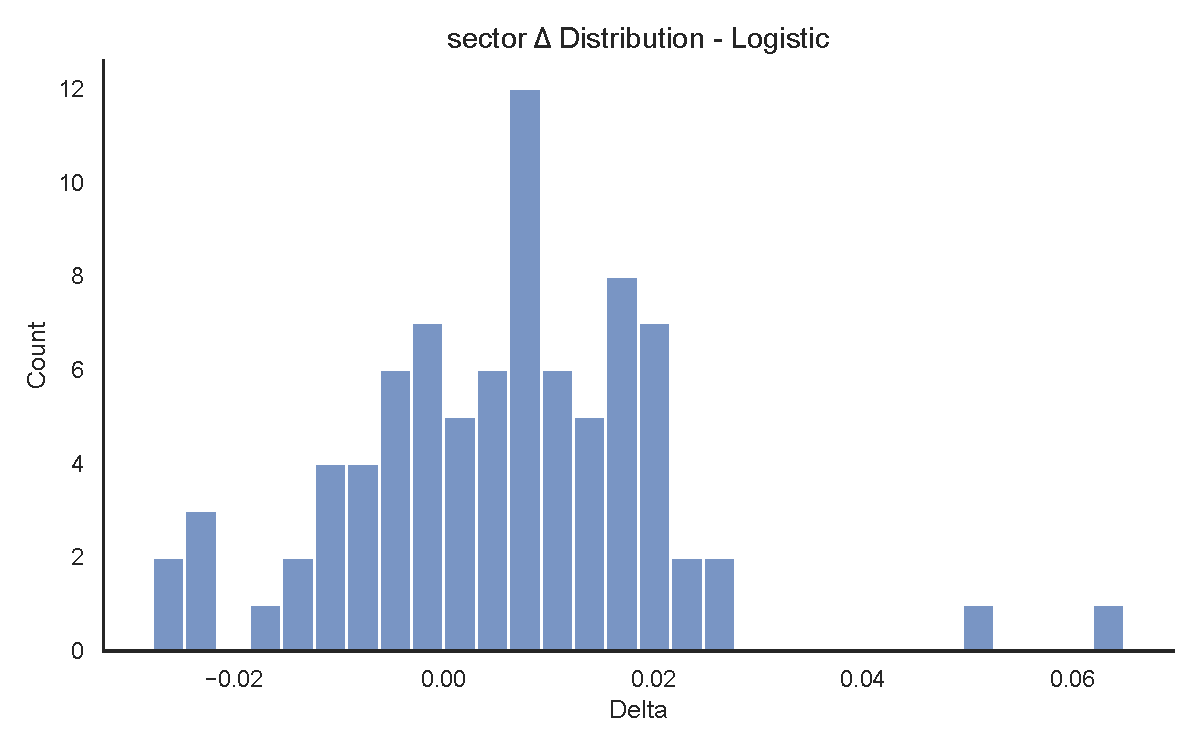
\includegraphics[width=\linewidth]{sector_grouping_comparison_images/sector_classification_delta_distribution_Logistic.pdf}
    \caption{Logistic}
\end{subfigure}
\hfill
\begin{subfigure}{0.32\textwidth}
    \centering
    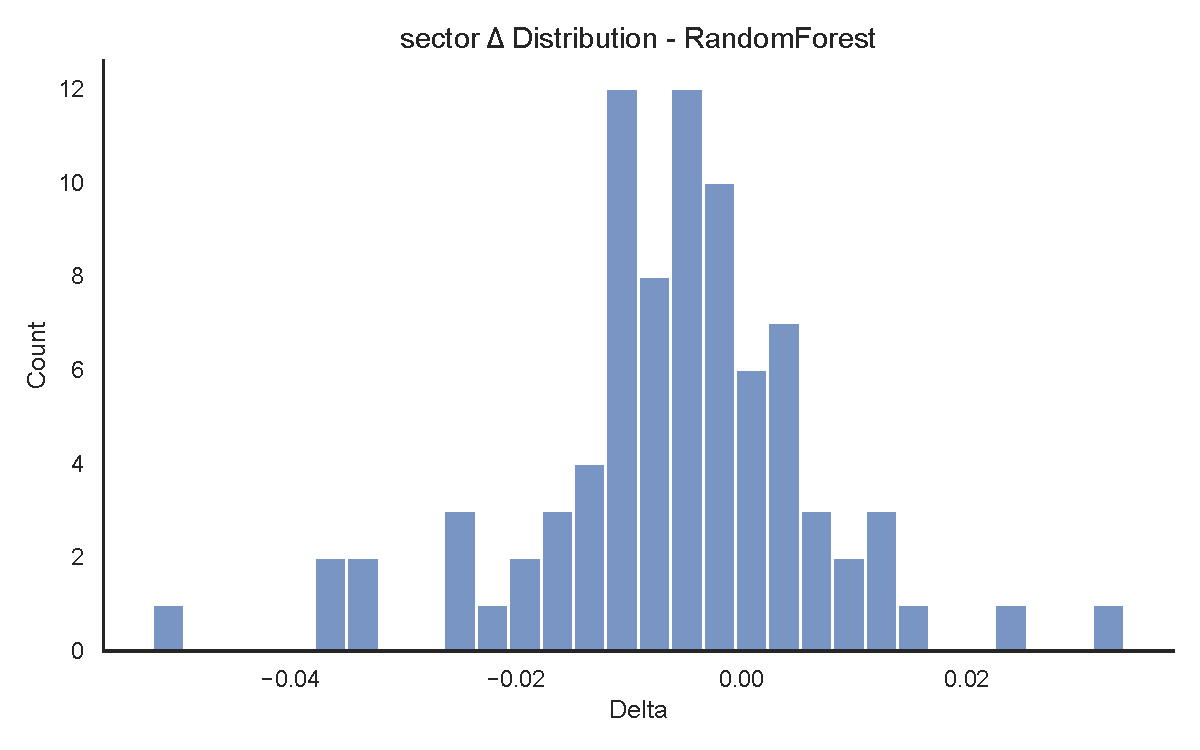
\includegraphics[width=\linewidth]{sector_grouping_comparison_images/sector_classification_delta_distribution_RandomForest.pdf}
    \caption{Random Forest}
\end{subfigure}
\hfill
\begin{subfigure}{0.32\textwidth}
    \centering
    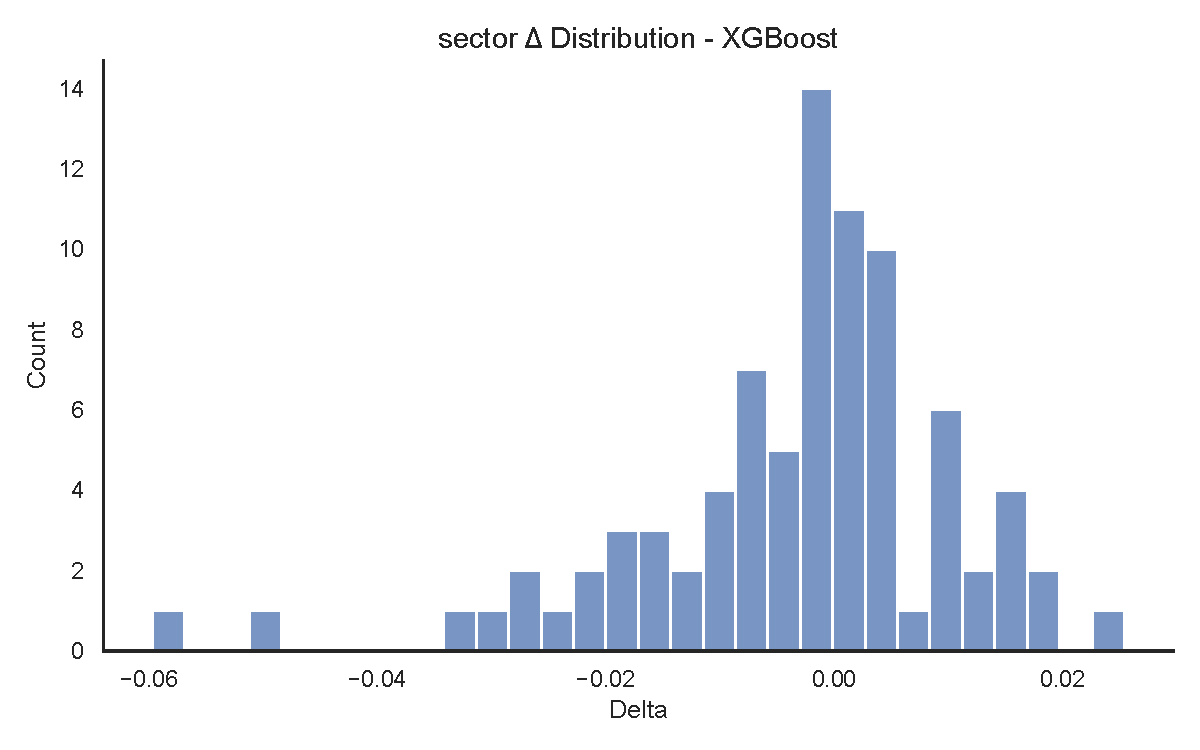
\includegraphics[width=\linewidth]{sector_grouping_comparison_images/sector_classification_delta_distribution_XGBoost.pdf}
    \caption{XGBoost}
\end{subfigure}

\vspace{0.35cm}

\textit{Classification}

\vspace{0.35cm}

% ----- Regression Row -----
\begin{subfigure}{0.32\textwidth}
    \centering
    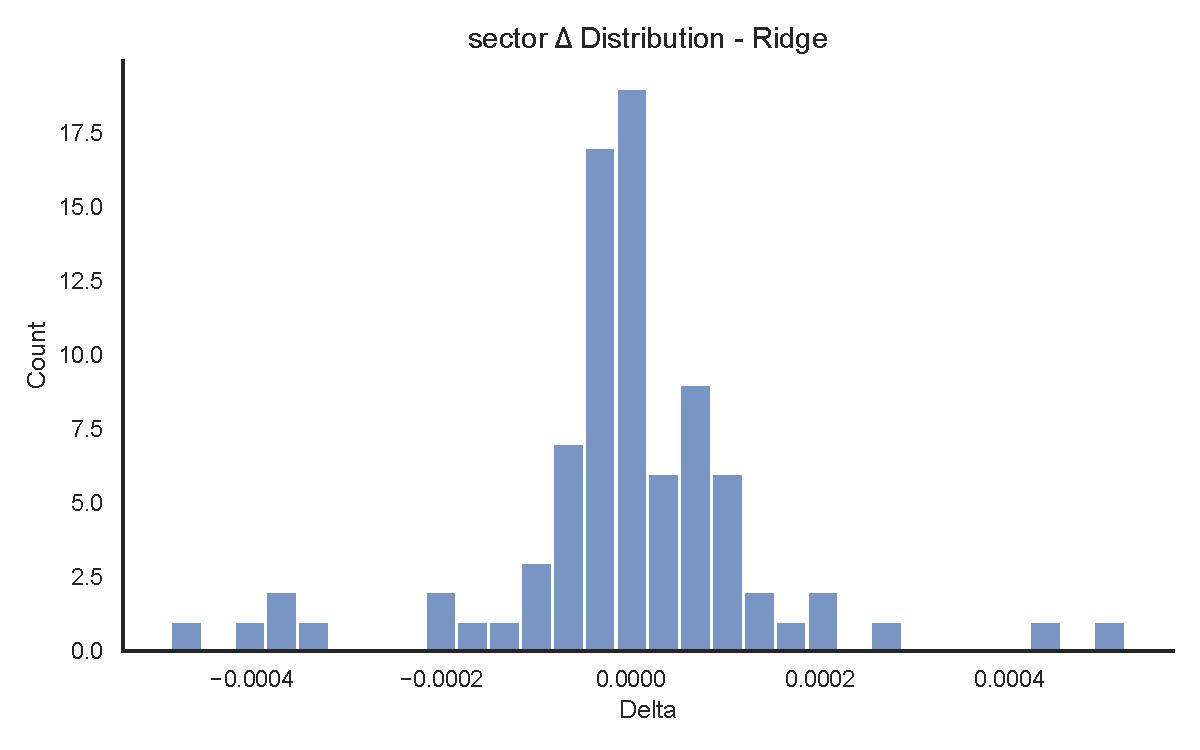
\includegraphics[width=\linewidth]{sector_grouping_comparison_images/sector_regression_delta_distribution_Ridge.pdf}
    \caption{Ridge}
\end{subfigure}
\hfill
\begin{subfigure}{0.32\textwidth}
    \centering
    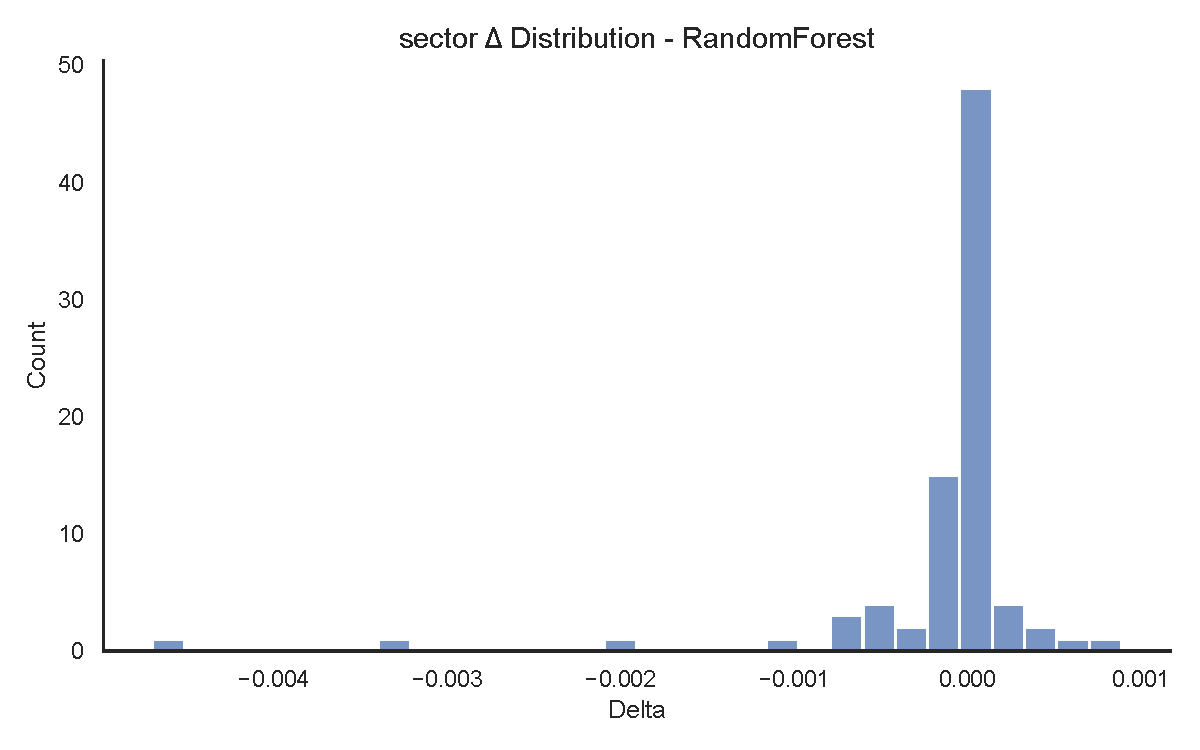
\includegraphics[width=\linewidth]{sector_grouping_comparison_images/sector_regression_delta_distribution_RandomForest.pdf}
    \caption{Random Forest}
\end{subfigure}
\hfill
\begin{subfigure}{0.32\textwidth}
    \centering
    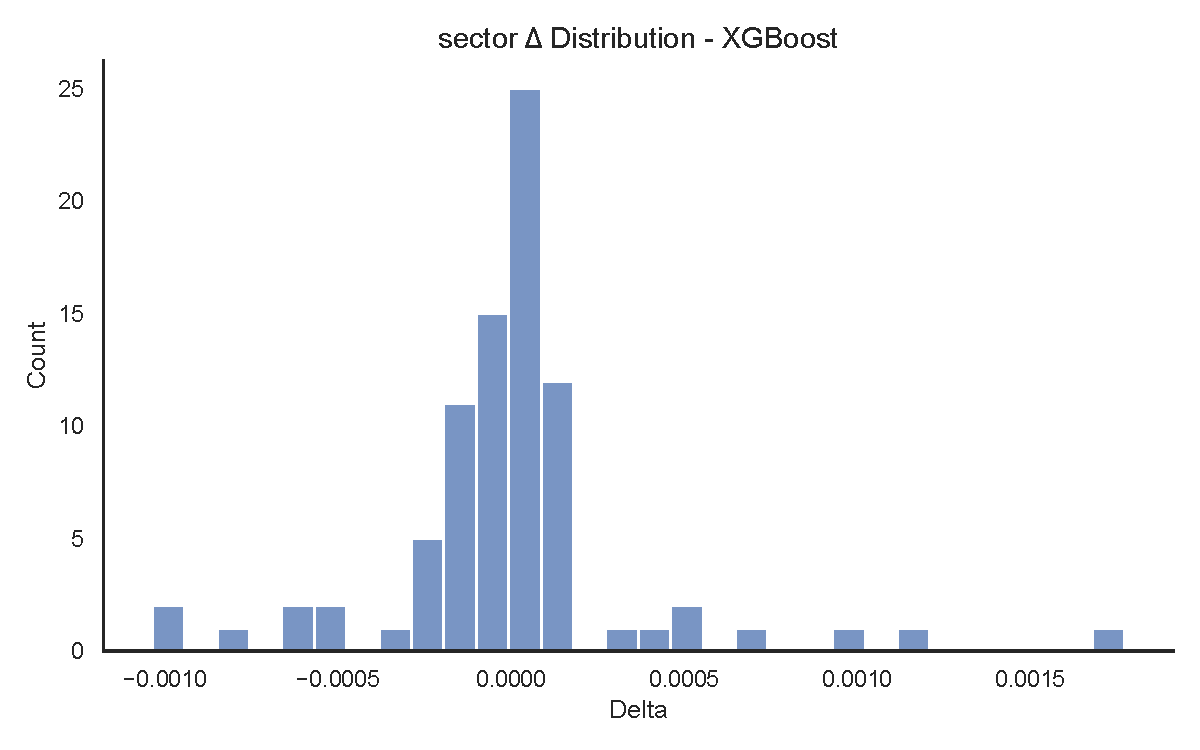
\includegraphics[width=\linewidth]{sector_grouping_comparison_images/sector_regression_delta_distribution_XGBoost.pdf}
    \caption{XGBoost}
\end{subfigure}

\vspace{0.35cm}

\textit{Regression}

\caption{Distribution of performance differences $\Delta$ between models trained with and without sentiment features for the sector-level experiments. Each histogram aggregates $\Delta$ values across all sectors and prediction horizons (1--7 days). The data is mostly concentrated around zero for regression, indicating negligible impact of sentiment features, while classification exhibits a wider spread with noticeable improvements for Logistic regression.}
\label{fig:sector_delta_distribution}
\end{figure}

\subsection{Industry-Level Results}

The industry-level experiments provide a different perspective due to the larger number of groups (97 industries). In this setting, the logistic regression model demonstrates a clear and statistically significant improvement when sentiment features are included. The average performance gain across industries is $\Delta = 0.0112$, with a $95\%$ confidence interval of $(0.0071, 0.0152)$ and highly significant $p$-values for both the $t$-test and Wilcoxon test ($p < 10^{-5}$). Furthermore, improvements are observed consistently across most prediction horizons, suggesting that sentiment signals extracted from financial reports carry meaningful predictive information within industry-specific contexts.

Random Forest exhibits the opposite behavior, showing a statistically significant decline in performance ($\Delta = -0.0038$ on average). XGBoost, on the other hand, shows no statistically significant difference between models trained with and without sentiment features.

The regression experiments at the industry level mirror the findings observed for sectors. Performance differences remain extremely small and generally lack statistical significance, regardless of the underlying model. This indicates that while sentiment may help classify directional movements of stock prices, it is less useful for accurately predicting the magnitude of short-term returns.

\begin{figure}
\centering

% ----- Classification Row -----
\begin{subfigure}{0.32\textwidth}
    \centering
    
\includegraphics[width=\linewidth]{sector_grouping_comparison_images/industry_classification_delta_distribution_Logistic.pdf}
    \caption{Logistic}
\end{subfigure}
\hfill
\begin{subfigure}{0.32\textwidth}
    \centering
    
\includegraphics[width=\linewidth]{sector_grouping_comparison_images/industry_classification_delta_distribution_RandomForest.pdf}
    \caption{Random Forest}
\end{subfigure}
\hfill
\begin{subfigure}{0.32\textwidth}
    \centering
    
\includegraphics[width=\linewidth]{sector_grouping_comparison_images/industry_classification_delta_distribution_XGBoost.pdf}
    \caption{XGBoost}
\end{subfigure}

\vspace{0.35cm}

\textit{Classification}

\vspace{0.35cm}

% ----- Regression Row -----
\begin{subfigure}{0.32\textwidth}
    \centering
    
\includegraphics[width=\linewidth]{sector_grouping_comparison_images/industry_regression_delta_distribution_Ridge.pdf}
    \caption{Ridge}
\end{subfigure}
\hfill
\begin{subfigure}{0.32\textwidth}
    \centering
    
\includegraphics[width=\linewidth]{sector_grouping_comparison_images/industry_regression_delta_distribution_RandomForest.pdf}
    \caption{Random Forest}
\end{subfigure}
\hfill
\begin{subfigure}{0.32\textwidth}
    \centering
    
\includegraphics[width=\linewidth]{sector_grouping_comparison_images/industry_regression_delta_distribution_XGBoost.pdf}
    \caption{XGBoost}
\end{subfigure}

\vspace{0.35cm}

\textit{Regression}

\caption{Distribution of performance differences $\Delta$ between models trained with and without sentiment features for the industry-level experiments. Each histogram aggregates $\Delta$ values across all industries and prediction horizons (1--7 days). The data is mostly concentrated around zero for regression, indicating negligible impact of sentiment features, while classification exhibits a wider spread with noticeable improvements for Logistic regression.}
\label{fig:industry_delta_distribution}
\end{figure}

\subsection{Company-Level Results}

Finally, the company-level experiments explore the most granular modeling scenario. Because each model is trained using data from a single company, the available number of samples is considerably smaller. As a result, the estimates of $\Delta$ display substantially higher variability and wider confidence intervals.

For logistic regression, the average improvement across companies is negative ($\Delta = -0.0111$), but the result is not statistically significant. The large variance across firms suggests that the usefulness of sentiment features may depend strongly on firm-specific factors such as disclosure style, investor attention, or market liquidity. Some companies exhibit substantial positive improvements, while others show performance degradation when sentiment features are included.

These findings highlight the limitations of company-level modeling under data constraints. While firm-specific models may capture idiosyncratic patterns, the limited number of filings per company reduces statistical reliability and increases the risk of overfitting.


\begin{figure}
\centering

% ----- Classification Row -----
\begin{subfigure}{0.32\textwidth}
    \centering
    
\includegraphics[width=\linewidth]{sector_grouping_comparison_images/ticker_classification_delta_distribution_Logistic.pdf}
    \caption{Logistic}
\end{subfigure}
\hfill
\begin{subfigure}{0.32\textwidth}
    \centering
    
\includegraphics[width=\linewidth]{sector_grouping_comparison_images/ticker_classification_delta_distribution_RandomForest.pdf}
    \caption{Random Forest}
\end{subfigure}
\hfill
\begin{subfigure}{0.32\textwidth}
    \centering
    
\includegraphics[width=\linewidth]{sector_grouping_comparison_images/ticker_classification_delta_distribution_XGBoost.pdf}
    \caption{XGBoost}
\end{subfigure}

\vspace{0.35cm}

\textit{Classification}

\vspace{0.35cm}

% ----- Regression Row -----
\begin{subfigure}{0.32\textwidth}
    \centering
    
\includegraphics[width=\linewidth]{sector_grouping_comparison_images/ticker_regression_delta_distribution_Ridge.pdf}
    \caption{Ridge}
\end{subfigure}
\hfill
\begin{subfigure}{0.32\textwidth}
    \centering
    
\includegraphics[width=\linewidth]{sector_grouping_comparison_images/ticker_regression_delta_distribution_RandomForest.pdf}
    \caption{Random Forest}
\end{subfigure}
\hfill
\begin{subfigure}{0.32\textwidth}
    \centering
    
\includegraphics[width=\linewidth]{sector_grouping_comparison_images/ticker_regression_delta_distribution_XGBoost.pdf}
    \caption{XGBoost}
\end{subfigure}

\vspace{0.35cm}

\textit{Regression}

\caption{Distribution of performance differences $\Delta$ between models trained with and without sentiment features for the company-level experiments. Each histogram aggregates $\Delta$ values across all companies and prediction horizons (1--7 days). The data exhibits a high degree of variability, due to the limiter number of samples available for each company.}
\label{fig:company_delta_distribution}
\end{figure}

\subsection{Discussion}

Taken together, the results of these experiments provide several important insights.

First, the effectiveness of sentiment features appears to depend strongly on the level of aggregation. Industry-level models show the most consistent improvements for classification tasks, suggesting that sentiment signals may capture industry-specific dynamics in how markets react to financial disclosures.

Second, the impact of sentiment features varies substantially across model classes. Linear models such as logistic regression appear to benefit the most from the inclusion of sentiment features, possibly because these models have limited capacity to extract nonlinear patterns from the structured market data alone. In contrast, tree-based models may already capture complex relationships within the existing feature set, leaving less room for additional improvement.

Finally, the company-level experiments highlight the trade-off between model specialization and data availability. While firm-specific models allow for highly tailored predictions, the limited number of observations per company introduces significant statistical noise, reducing the reliability of the estimated effects.

\section{Time-Series Models: LSTM and PatchTST Experiments}

\subsection{Company-Level Results}

This section presents the results of time-series models trained at the company (ticker) level. Both an LSTM architecture and a PatchTST transformer model are evaluated across multiple sequence lengths. The goal is to determine whether modeling temporal dependencies between filings improves predictive performance and whether sentiment features provide additional value in this setting. Results are reported separately for classification and regression tasks, and statistical significance is assessed using paired tests across tickers.

\subsubsection{Classification Results}

For the classification task, the LSTM model with a sequence length of five filings yields the most consistent and statistically significant improvements. In particular, for the three-day prediction horizon, the model achieves a mean increase in macro F1 score of $\Delta = 0.065189$, with a statistically significant $p$-value of $0.005$ and a $95\%$ confidence interval of $(0.026322, 0.104056)$. When averaged across all horizons, the overall improvement remains positive at $\Delta = 0.022016$, which is also statistically significant. The effect is heterogeneous across companies, with ticker WES showing the largest improvement of $0.091123$, while USAC exhibits degraded performance with $\Delta = -0.042443$. These results suggest that short temporal sequences allow the LSTM model to exploit recent sentiment dynamics effectively.

Increasing the sequence length to ten filings results in substantially weaker evidence. Although the mean overall improvement remains positive at $\Delta = 0.005274$, the associated $p$-values are large across all horizons, indicating that the effect is not statistically significant. The dispersion across companies also increases, with WES showing a strong improvement of $0.235125$, while EME experiences a degradation of $-0.156716$. This behaviour suggests that longer sequences introduce additional noise and reduce the consistency of the sentiment signal.

For a sequence length of fifteen filings, statistically significant improvement is observed only for the one-day horizon, where the mean increase reaches $\Delta = 0.067540$. However, the overall mean improvement of $\Delta = 0.003242$ is not statistically significant. The best-performing ticker in this setting is WES with an improvement of $0.077631$, while DLR shows degraded performance with $\Delta = -0.067193$. A similar pattern is observed for a sequence length of twenty filings, where the overall mean improvement is $\Delta = 0.013408$, but none of the horizons reach statistical significance. The largest improvement is observed for JEF with $0.089934$, whereas NWN shows a decrease of $-0.085640$. Overall, these results indicate that the LSTM model benefits primarily from shorter temporal contexts.

The PatchTST model displays weaker and less consistent behaviour in the classification setting. With a sequence length of five filings, the mean overall improvement is $\Delta = 0.003906$, but all horizons exhibit large $p$-values, indicating a lack of statistical significance. The best-performing ticker is WES with an improvement of $0.052816$, while GSBD shows degraded performance of $-0.081072$. For a sequence length of ten filings, most horizons again display high $p$-values, although the one-day horizon shows a statistically significant degradation with mean $\Delta = -0.058218$. The extremes range from an improvement of $0.115539$ for MGEE to a degradation of $-0.064966$ for MLR.

For sequence lengths of fifteen and twenty filings, the PatchTST model does not produce statistically significant results across any horizon. At a sequence length of fifteen, the largest improvement is observed for WES with $0.128477$, while MLR shows a degradation of $-0.103806$. At a sequence length of twenty, JEF achieves an improvement of $0.089934$, whereas NWN exhibits degraded performance with $\Delta = -0.085640$. Overall, the transformer-based model appears less effective than the LSTM for classification at the ticker level, particularly for shorter temporal contexts.

\subsubsection{Regression Results}

For the regression task, the LSTM model generally fails to produce statistically significant improvements. With a sequence length of five filings, all horizons display large $p$-values. Although not statistically significant, the mean overall change in RMSE is $\Delta = 0.001470$, indicating degraded performance when sentiment features are included. The best-performing ticker is JEF with $\Delta = -0.013684$, while RHI exhibits degraded performance with $\Delta = 0.021053$. A similar pattern is observed for a sequence length of ten filings, where the overall effect remains negative and statistically insignificant. In this setting, WES shows an improvement of $-0.013941$, whereas RHI again exhibits degraded performance with $0.028058$.

For a sequence length of fifteen filings, statistically significant degradation is observed for the six-day horizon, with a mean increase in RMSE of $\Delta = 0.011960$. The overall effect remains inconsistent across companies, with JEF showing improved performance of $-0.010757$ and GSBD displaying degraded performance of $0.024234$. At a sequence length of twenty filings, all horizons again exhibit high $p$-values. The extremes range from an improvement of $-0.014657$ for USAC to a degradation of $0.039314$ for DLR. These results suggest that the LSTM model does not benefit from sentiment features for numerical return prediction at the company level.

In contrast, the PatchTST model shows stronger behaviour for short sequences in the regression task. With a sequence length of five filings, the one-day horizon exhibits a statistically significant improvement with mean $\Delta = -0.158464$. The mean overall effect across horizons is also statistically significant at $\Delta = -0.056178$, indicating improved predictive performance. The best-performing ticker is JEF with $\Delta = -0.180596$, while NWN shows degraded performance with $0.083941$. This suggests that the transformer architecture can effectively leverage short-term temporal sentiment patterns for return prediction.

However, for longer sequence lengths, the PatchTST model again exhibits high $p$-values across all horizons. With a sequence length of ten filings, the extremes range from an improvement of $-0.281058$ for XRX to a degradation of $0.176403$ for WES. For a sequence length of fifteen filings, GSBD shows strong improvement of $-0.296095$, while DLR exhibits degraded performance of $0.318635$. At a sequence length of twenty filings, NWN achieves improvement of $-0.284585$, whereas XRX shows degraded performance of $0.420942$. Despite these large individual effects, the lack of statistical significance indicates that the improvements are not consistent across companies.

Overall, the ticker-level time-series experiments suggest that temporal modeling provides limited but task-dependent benefits. For classification, short LSTM sequences yield the most consistent improvements, while longer contexts reduce statistical significance. For regression, the PatchTST model with short sequences provides the strongest evidence of improvement, whereas the LSTM model generally fails to benefit from sentiment features. These results indicate that temporal dependencies between filings are most informative over short horizons and that transformer-based architectures may better capture these effects for numerical return prediction.

\begin{figure}
\centering
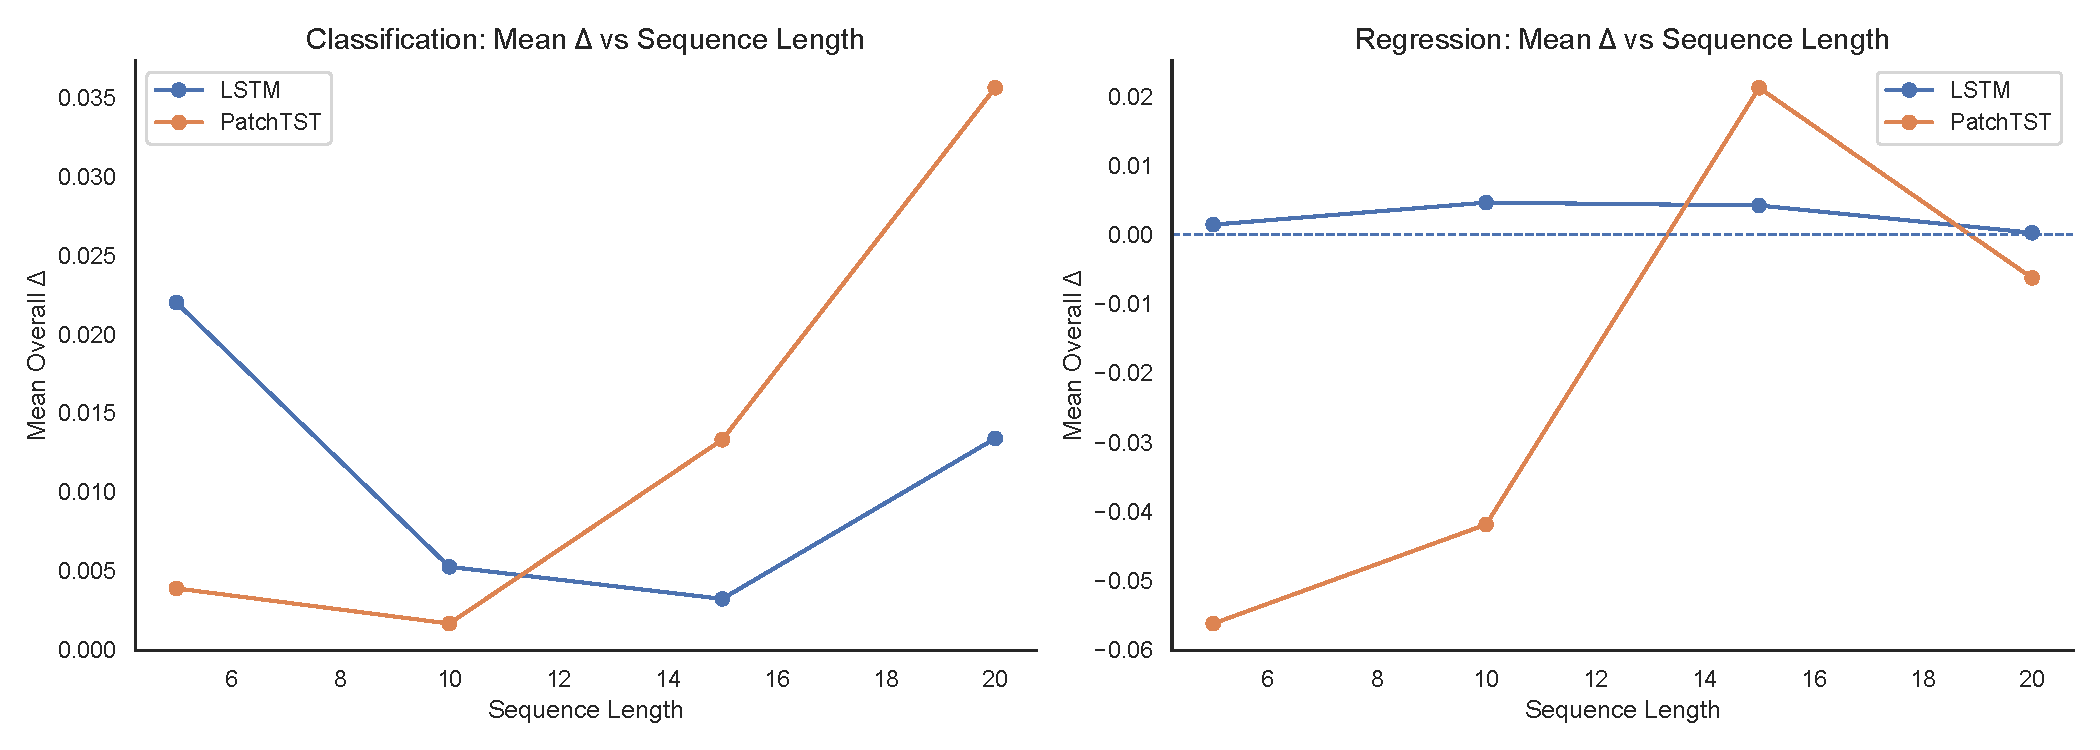
\includegraphics[width=0.8\textwidth]{time_series/ticker_sequence_length_model_comparison.pdf}
\caption{Evolution of the mean overall delta across all the prediction horizons against sequence length. The LSTM and PatchTST models were trained and evaluated at the company level.}
\label{fig:ticker_sequence_length_comparison}
\end{figure}

\subsection{Sector-Level Results}

This section presents the results of the time-series experiments performed at the sector level. In this setting, filings are aggregated by sector and ordered chronologically, allowing both LSTM and PatchTST models to capture temporal dependencies in sentiment dynamics at a broader market level. The objective is to evaluate whether temporal modelling improves predictive performance and whether sentiment features contribute meaningful information when analyzed at the sector granularity. Results are reported separately for classification and regression tasks, and statistical significance is assessed across sectors.

\subsubsection{Classification Results}

For the classification task, the LSTM model with a sequence length of five filings exhibits modest but partially significant improvements. A statistically significant increase in macro F1 score is observed for the two-day prediction horizon, with a mean improvement of $\Delta = 0.028080$. However, the mean overall improvement across all horizons is smaller, $\Delta = 0.005386$, and does not reach statistical significance. The effect varies across sectors, with the Health Care sector showing the largest improvement of $0.044555$, while the Utilities sector experiences degraded performance with $\Delta = -0.033524$. These results suggest that short sequences provide limited but potentially useful temporal information at the sector level.

Increasing the sequence length to ten filings results in weaker evidence. The LSTM model displays high $p$-values across all horizons, indicating that the observed differences are not statistically significant. Nevertheless, variability across sectors remains noticeable, with Finance showing an improvement of $0.051385$, while Consumer Staples exhibits a degradation of $-0.019872$. This behaviour suggests that longer sequences may introduce additional variability without consistent gains.

Stronger results are obtained when the sequence length is increased to fifteen filings. In this configuration, statistically significant improvements are observed for the one-day and five-day horizons, with mean increases of $\Delta = 0.061776$ and $\Delta = 0.025550$, respectively. The mean overall improvement across all horizons is $\Delta = 0.016668$, which is also statistically significant. At the sector level, Telecommunications displays the largest improvement of $0.073402$, while Technology shows a small degradation of $-0.018192$. These findings indicate that intermediate temporal contexts allow the LSTM model to capture sector-level sentiment dynamics more effectively.

A similar pattern is observed for a sequence length of twenty filings. The LSTM model achieves statistically significant improvements for the two-day and seven-day horizons, with mean increases of $\Delta = 0.034196$ and $\Delta = 0.029745$, respectively. The overall mean improvement across horizons is $\Delta = 0.010992$, which is also statistically significant. The Energy sector shows the largest improvement of $0.041678$, whereas the Technology sector again exhibits degraded performance with $\Delta = -0.026257$. These results suggest that the LSTM model benefits from longer sector-level sequences, although the magnitude of improvement remains moderate.

In contrast, the PatchTST model does not produce statistically significant improvements in the classification setting. For a sequence length of five filings, all horizons display high $p$-values, with the Technology sector showing the largest improvement of $0.043503$ and the Miscellaneous sector exhibiting degraded performance of $-0.045510$. With a sequence length of ten filings, the results remain statistically insignificant, with extremes ranging from an improvement of $0.029958$ for Industrials to a degradation of $-0.024859$ for Energy.

For sequence lengths of fifteen and twenty filings, the PatchTST model again fails to achieve statistical significance. At a sequence length of fifteen, the Energy sector shows the largest improvement of $0.057647$, while Real Estate displays degraded performance of $-0.042957$. With a sequence length of twenty, Consumer Discretionary achieves an improvement of $0.027943$, whereas Finance exhibits degraded performance of $-0.027644$. Overall, the transformer-based architecture appears less effective than the LSTM model for sector-level classification, particularly in terms of statistical consistency across sectors.

\subsubsection{Regression Results}

For the regression task, the LSTM model consistently displays degraded performance when sentiment features are included. With a sequence length of five filings, the mean overall change in RMSE is $\Delta = 0.001738$, which represents a statistically significant degradation. The Industrials sector shows the largest improvement with $\Delta = -0.001558$, while Real Estate experiences degraded performance of $0.004865$. A similar pattern is observed for a sequence length of ten filings, where the mean overall change is $\Delta = 0.001025$, again statistically significant. The extremes range from an improvement of $-0.001578$ for Industrials to a degradation of $0.004104$ for Basic Materials.

For a sequence length of fifteen filings, the LSTM model continues to display statistically significant degradation, with a mean overall change of $\Delta = 0.001940$. The Finance sector shows improved performance with $\Delta = -0.002218$, whereas Consumer Discretionary exhibits degraded performance of $0.008853$. When the sequence length is increased to twenty filings, the results become statistically insignificant, with high $p$-values across all horizons. The extremes range from an improvement of $-0.002462$ for Energy to a degradation of $0.003616$ for Industrials. These results indicate that sector-level temporal modeling with LSTM does not improve return prediction and may introduce additional noise.

The PatchTST model exhibits mixed behaviour in the regression setting. With a sequence length of five filings, the mean overall change is $\Delta = -0.002801$, suggesting improved performance, but the effect is not statistically significant. The Finance sector shows the largest improvement of $-0.103430$, while Energy exhibits degraded performance of $0.154796$. For a sequence length of ten filings, all horizons again display high $p$-values. The extremes range from an improvement of $-0.182050$ for Consumer Staples to a degradation of $0.059769$ for Real Estate.

For a sequence length of fifteen filings, the PatchTST model produces statistically significant improvement for the three-day horizon, with a mean change of $\Delta = -0.175542$. The Telecommunications sector shows the largest improvement of $-0.189693$, while Real Estate exhibits degraded performance of $0.106971$. However, the overall effect across horizons remains statistically insignificant. With a sequence length of twenty filings, the results again display high $p$-values across all horizons. The extremes range from an improvement of $-0.124313$ for Finance to a degradation of $0.163330$ for Technology.

Overall, the sector-level experiments indicate that temporal modeling provides moderate benefits for classification but limited value for regression. The LSTM model benefits from intermediate and longer sequence lengths in the classification task, suggesting that sector-level sentiment dynamics evolve over multiple filings. In contrast, regression performance generally deteriorates when sentiment features are incorporated, particularly for the LSTM model. The PatchTST transformer exhibits weaker and less consistent behaviour overall, with only isolated improvements observed for specific horizons. These findings suggest that sector-level temporal dependencies are more informative for directional classification than for numerical return prediction.

\begin{figure}
\centering
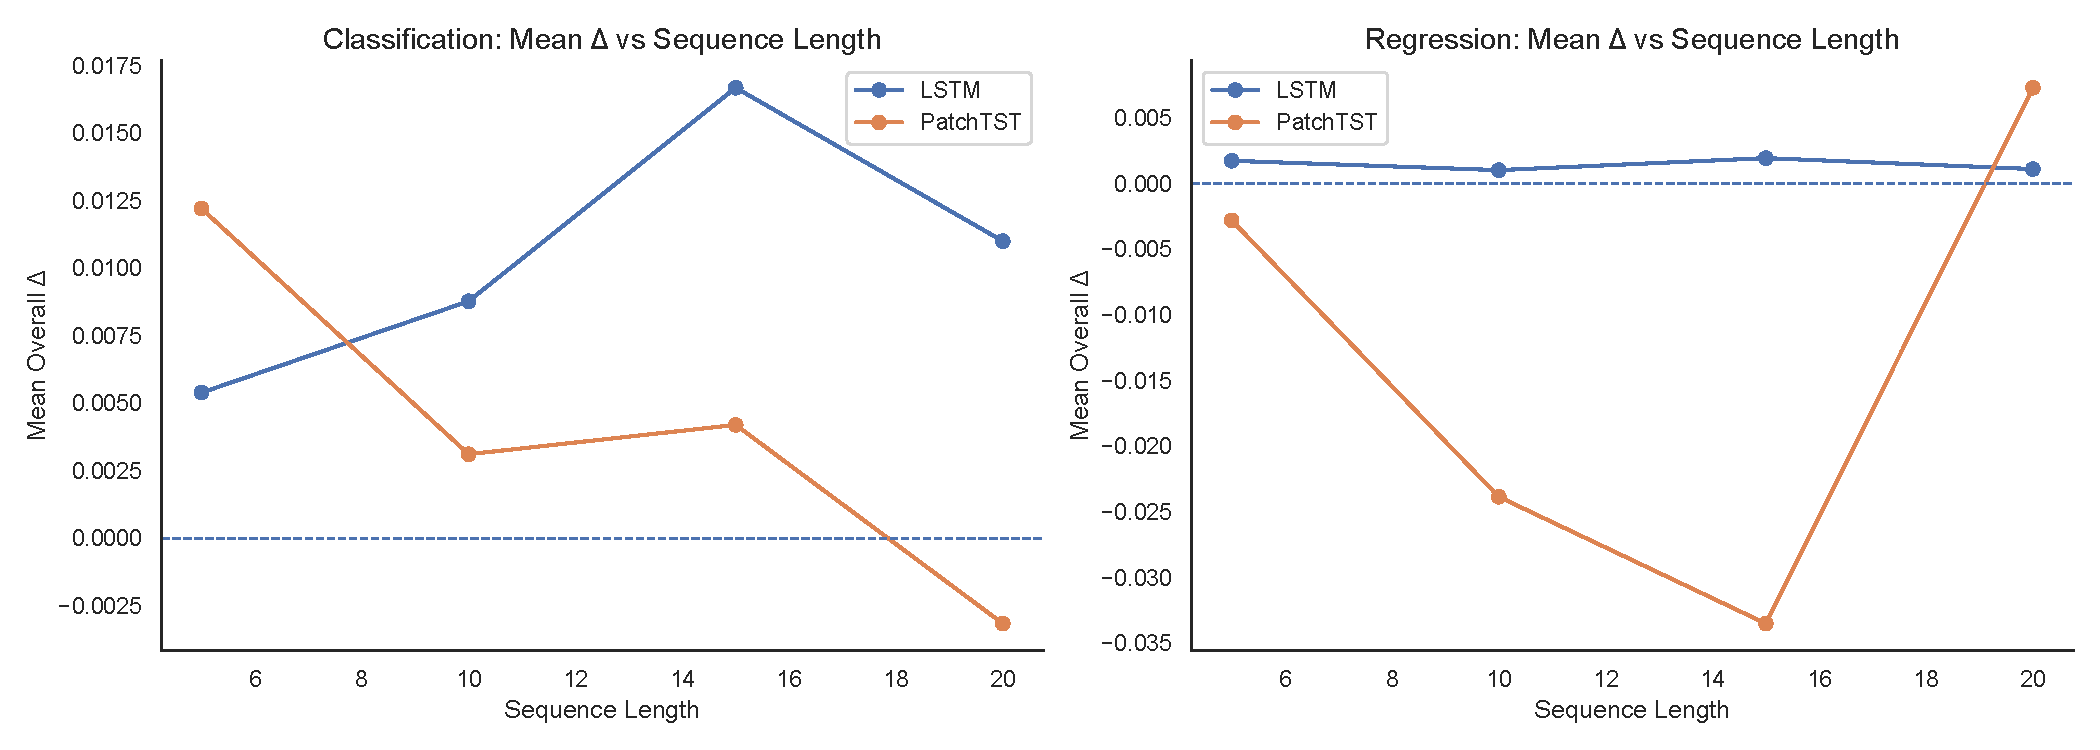
\includegraphics[width=0.8\textwidth]{time_series/sector_sequence_length_model_comparison.pdf}
\caption{Evolution of the mean overall delta across all the prediction horizons against sequence length. The LSTM and PatchTST models were trained and evaluated at the sector level.}
\label{fig:sector_sequence_length_comparison}
\end{figure}

\subsection{Industry-Level Results}

This section presents the results of the time-series experiments performed at the industry level. Compared to sector-level aggregation, industry grouping provides a finer granularity while still allowing temporal dependencies between filings to be modeled across multiple firms. Both LSTM and PatchTST architectures are evaluated across multiple sequence lengths, and the impact of sentiment features is assessed using paired statistical tests across industries. Results are reported separately for classification and regression tasks.

\subsubsection{Classification Results}

For the classification task, the LSTM model consistently exhibits statistically significant improvements across all tested sequence lengths. With a sequence length of five filings, a statistically significant improvement is observed for the six-day prediction horizon, with a mean increase in macro F1 score of $\Delta = 0.017768$. The mean overall improvement across all horizons is also statistically significant at $\Delta = 0.009922$. The effect varies across industries, with Cable \& Other Pay Television Services showing the largest improvement of $0.093778$, while the Precious Metals industry exhibits degraded performance with $\Delta = -0.068252$. These results indicate that short temporal contexts already provide useful predictive information at the industry level.

Increasing the sequence length to ten filings yields stronger and more consistent improvements. Statistically significant gains are observed for the one-day and seven-day horizons, with mean increases of $\Delta = 0.017355$ and $\Delta = 0.030988$, respectively. The overall mean improvement across all horizons is also statistically significant at $\Delta = 0.012175$. The largest improvement is observed for the Consumer Electronics/Appliances industry with $0.090481$, while the Ophthalmic Goods industry shows degraded performance with $\Delta = -0.100061$. These results suggest that moderate sequence lengths allow the LSTM model to capture richer temporal sentiment dynamics within industries.

For a sequence length of fifteen filings, statistically significant improvement is observed for the one-day horizon with $\Delta = 0.020544$. The mean overall improvement remains statistically significant at $\Delta = 0.009590$. The Farming/Seeds/Milling industry shows the largest improvement of $0.107958$, whereas Wholesale Distributors exhibit degraded performance with $\Delta = -0.122487$. When the sequence length is increased to twenty filings, statistically significant improvements are again observed for the one-day and seven-day horizons, with $\Delta = 0.016587$ and $\Delta = 0.021185$, respectively. The overall mean improvement across horizons is $\Delta = 0.011102$, also statistically significant. The largest improvement is observed for Meat/Poultry/Fish with $0.117101$, while Ophthalmic Goods again displays degraded performance with $\Delta = -0.065267$. Overall, the LSTM model demonstrates consistent and statistically significant gains across all tested sequence lengths in the industry-level classification setting.

The PatchTST model also produces statistically significant improvements for several sequence lengths, although the effects are generally smaller than those observed for the LSTM model. With a sequence length of five filings, statistically significant improvement is observed for the five-day horizon with $\Delta = 0.021053$, and the mean overall improvement across horizons is also significant at $\Delta = 0.006295$. The largest improvement is observed for Paints/Coatings with $0.098751$, while Commercial Banks exhibit degraded performance with $\Delta = -0.165768$.

For a sequence length of ten filings, statistically significant improvement is observed for the seven-day horizon with $\Delta = 0.012564$, and the mean overall improvement across horizons is $\Delta = 0.005371$. The Computer Communications Equipment industry shows the largest improvement of $0.116364$, whereas Accident \& Health Insurance exhibits degraded performance with $\Delta = -0.068147$. With a sequence length of fifteen filings, the mean overall delta of $\Delta = 0.004835$ remains statistically significant, although no individual horizons show strong effects. The largest improvement is observed for Oil and Gas Field Machinery with $0.069994$, while Pollution Control Equipment displays degraded performance with $\Delta = -0.064798$. For a sequence length of twenty filings, the PatchTST model does not produce statistically significant results. The extremes range from an improvement of $0.094195$ for Cable \& Other Pay Television Services to a degradation of $-0.127700$ for Meat/Poultry/Fish. Overall, the transformer-based model provides modest but consistent improvements for shorter and intermediate sequence lengths, although the magnitude of gains is smaller than for the LSTM model.

\subsubsection{Regression Results}

For the regression task, the LSTM model consistently displays statistically significant degradation in predictive performance when sentiment features are included. With a sequence length of five filings, statistically significant degradation is observed for the one-day horizon, with $\Delta = 0.002515$. The extremes range from an improvement of $-0.049705$ for Commercial Banks to a degradation of $0.019540$ for Steel/Iron Ore. For a sequence length of ten filings, the mean overall delta is $\Delta = 0.001484$, indicating statistically significant degradation. The largest improvement is observed for Wholesale Distributors with $-0.016837$, while Coal Mining exhibits degraded performance with $0.026571$.

Similar behaviour is observed for longer sequence lengths. With fifteen filings, the mean overall delta is $\Delta = 0.001509$, again statistically significant. Office Equipment/Supplies/Services shows improved performance with $-0.010640$, whereas Wholesale Distributors display degraded performance of $0.012404$. For a sequence length of twenty filings, the mean overall delta remains statistically significant at $\Delta = 0.001025$. The extremes range from an improvement of $-0.014092$ for Accident \& Health Insurance to a degradation of $0.011117$ for Medical Electronics. These results indicate that temporal modeling with LSTM does not improve numerical return prediction at the industry level and may introduce additional noise.

In contrast, the PatchTST model produces several statistically significant improvements for shorter sequence lengths. With a sequence length of five filings, statistically significant improvements are observed for the two-day and seven-day horizons, with $\Delta = -0.038129$ and $\Delta = -0.036723$, respectively. The mean overall improvement across all horizons is also statistically significant at $\Delta = -0.016597$. The Water Supply industry shows the largest improvement of $-0.196339$, while Other Consumer Services exhibit degraded performance with $0.153214$.

For a sequence length of ten filings, statistically significant improvement is observed for the one-day horizon with $\Delta = -0.042393$. The largest improvement is observed for Aluminum with $-0.225476$, whereas Clothing/Shoe/Accessory Stores display degraded performance with $0.228436$. With a sequence length of fifteen filings, the PatchTST model does not produce statistically significant results, although large variations across industries remain. The extremes range from an improvement of $-0.242642$ for Advertising to a degradation of $0.294257$ for Meat/Poultry/Fish. For a sequence length of twenty filings, statistically significant degradation is observed for the five-day horizon with $\Delta = 0.046109$. The extremes range from an improvement of $-0.252129$ for Shoe Manufacturing to a degradation of $0.241827$ for Auto Parts: O.E.M.

Overall, the industry-level time-series experiments indicate that temporal modeling is most beneficial for classification tasks. The LSTM model provides consistent and statistically significant improvements across all sequence lengths, suggesting that industry-level sentiment dynamics contain useful directional information. For regression, however, the LSTM model consistently degrades performance, while the PatchTST model provides improvements primarily for shorter sequences. These findings suggest that temporal sentiment dependencies at the industry level are more informative for directional prediction than for numerical return estimation, and that transformer-based architectures may better capture short-term return dynamics in this setting.

\begin{figure}
\centering
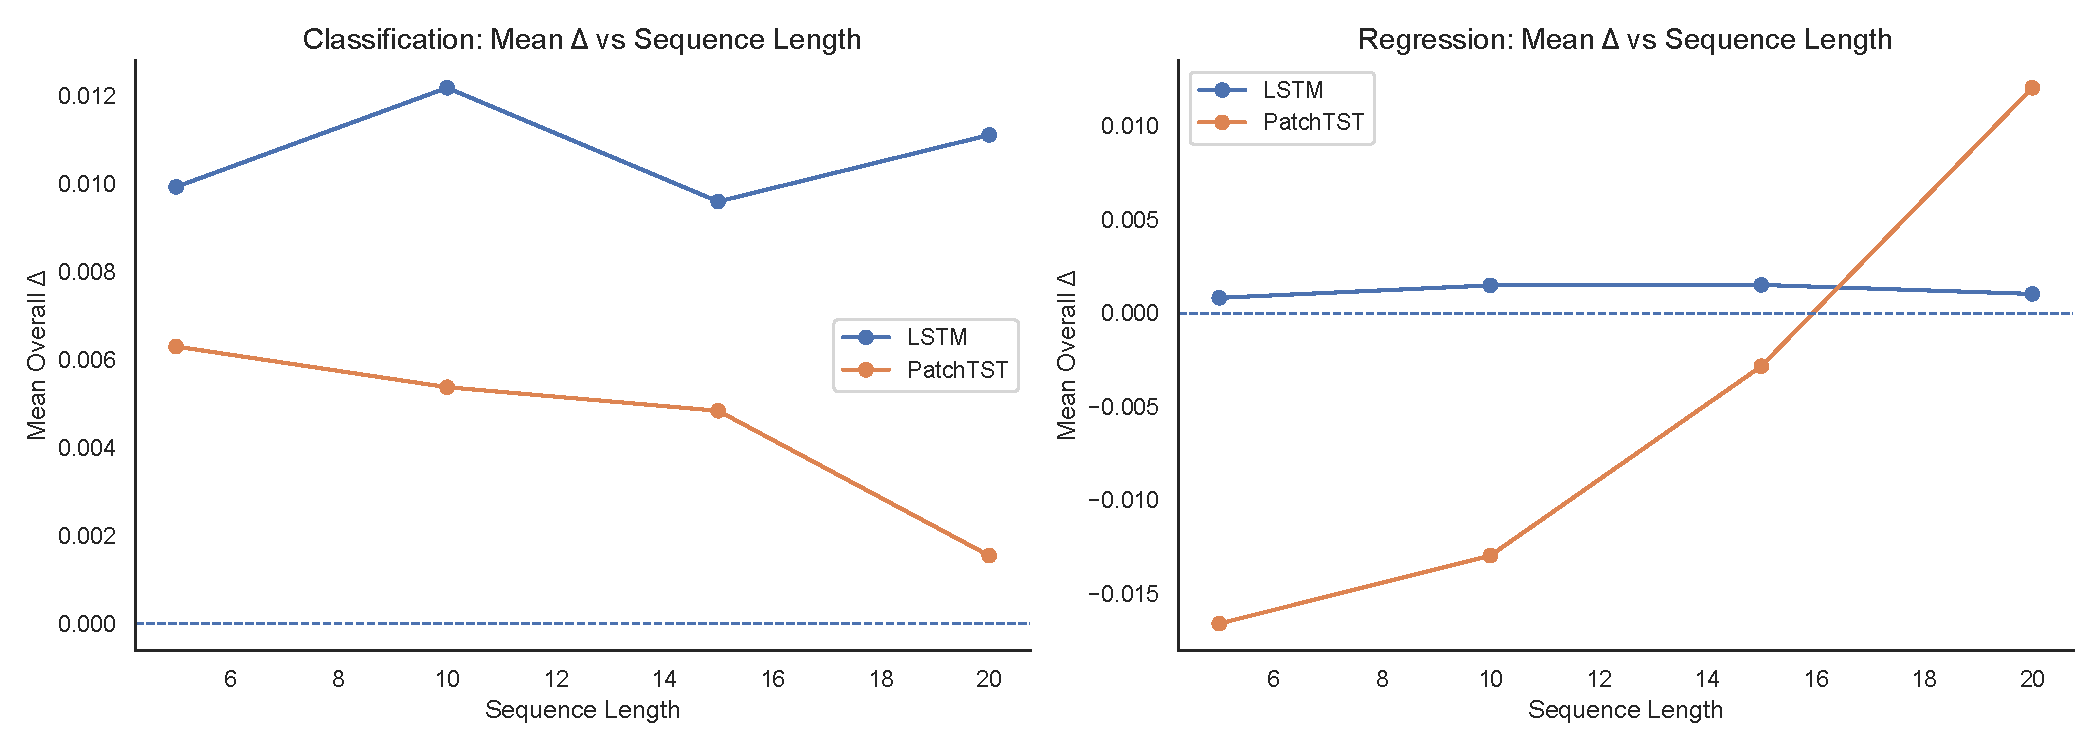
\includegraphics[width=0.8\textwidth]{time_series/industry_sequence_length_model_comparison.pdf}
\caption{Evolution of the mean overall delta across all the prediction horizons against sequence length. The LSTM and PatchTST models were trained and evaluated at the industry level.}
\label{fig:industry_sequence_length_comparison}
\end{figure}